\documentclass[a4paper, 12p]{article}
\usepackage[spanish]{babel} 
\usepackage{amsmath} 
\usepackage[colorlinks=true]{hyperref}
\usepackage{enumitem} 
\usepackage{graphicx}   
\usepackage[a4paper,top=3cm,bottom=3cm,left=3cm,right=3cm,marginparwidth=1.75cm]{geometry} 
\usepackage[]{subfigure}
\graphicspath{{./graficos/Lab-Termo/Git/Documentos}} 
\usepackage{float}
%\usepackage[]{txfonts}
\usepackage{multicol}



\newenvironment{Figura}
{\par\medskip\noindent\minipage{\linewidth}}
{\endminipage\par\medskip}

%==================================================================================
\begin{document}
\begin{titlepage}
      \begin{center}     
              
            %
\includegraphics[width=0.2\textwidth]{graficos/escudo_udec.png}                       %Para poner logo udec   %{nombre carpeta\nombreimagen}
            
            
            
            \vspace{1cm}
            \textsc{{\LARGE Universidad de Concepción}}
            
            \vspace{1cm}
            {\scshape\Large Facultad de ciencias fisícas y matemáticas \par}
            \vspace{2cm}
            {\scshape\Huge Laboratorio 1 \par}
            \vspace{2cm}
            {\itshape\Large Proyecto laboratorio termodinámica \par}
            \vfill
            {\Large Autores: \par}
            {\Large Martina Contreras, Noemí De la peña, Benjamín Opazo. \par}
            \vfill
            \vfill
            {\Large Profesor: \par}
            {\Large Claudio Alonso Faúndez Araya \par}
            \vfill
            \vfill
            {\Large Carrera: \par}
            {\Large Ciencias fisícas \par}
            \vfill
            \vfill
            {\Large Ayudantes: \par}
            {\Large Arelly Nunez y Anahis Verana \par}
            \vfill
            {\Large Octubre 2022 \par}
      \end{center}
\end{titlepage}            
%\maketitle  

\tableofcontents
\newpage

%========Introducción
\section{Introdución}



%=========Marco Teórico
\section{Marco Teórico}



%=========Materiales


\section{Materiales}
\begin{itemize}
      \item Termómetro digital
      \item Vaso precipitado
      \item Estufa eléctrica agua
      \item Alcohol etílico
      \item Benceno
\end{itemize}






\section{Procedimiento y Resultados}
%%%%%%GRAFICOS%%%%%%%%
% \begin{figure}[H]      
%             \begin{subfigure}
%                   \raggedright
%                   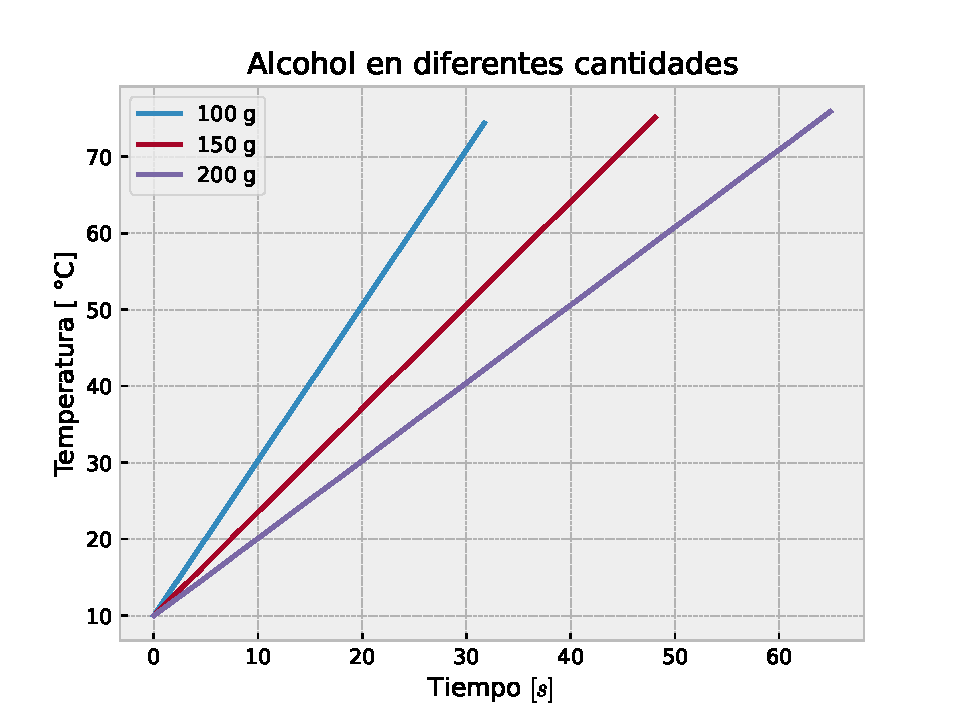
\includegraphics[width=8cm, height=6cm]{masa/grafico-alcohol-masa.pdf}
%             \end{subfigure}
%       \begin{subfigure}
%                   \raggedright
%                   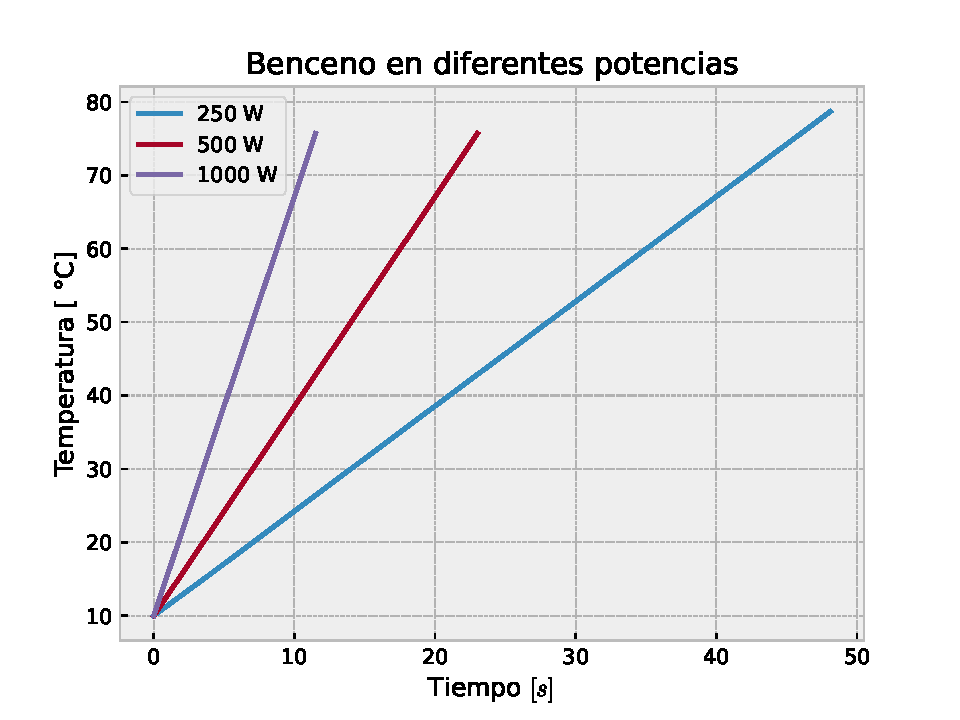
\includegraphics[width=8cm, height=6cm]{potencia/grafico-benceno-potencia.pdf}
%             \end{subfigure}
%             \begin{subfigure}
%                   \raggedright
%                   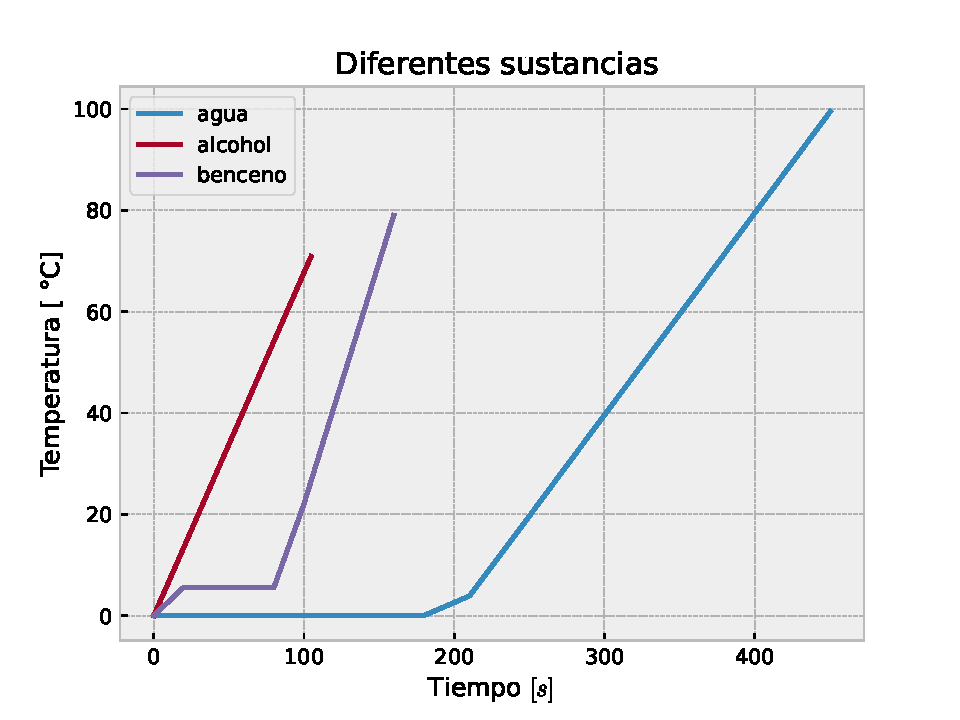
\includegraphics[width=8cm, height=6cm]{naturaleza/grafico-naturaleza-sustancias.pdf}
%             \end{subfigure}
% \end{figure}






\subsection{Determinación puntos de fusión y de ebullición}
\begin{itemize}
      \item Primero, seleccionaremos una potencia de 250 [W], una masa de 150[g] de agua y una temperatura inicial de -10°C.
      \item Segundo, anotamos la temperatura, hasta llegar al punto de ebullición.
      \item Tercero, realizamos lo mismo para el alcohol y el benceno.
      \item Finalmente, hacemos un gráfico de temperatura vs tiempo para los datos obtenidos.
\end{itemize}


\begin{table}[H]
      \centering
      \begin{tabular}{|c|c|c|}\hline
            Sustancia [g]& Tiempo [s] & Temperatura [°C]\\ \hline
                          &    0     &  0\\
                          &     1.7  & -8.6\\
                          &   30.9   & 0\\
                          &   60.1   & 0\\
                          &   93.7   & 0\\
                          &   99.1   & 0\\
                          &   120.1  & 0\\
                          &   149.8  & 0\\
             agua         &   180.2  & 0\\
                          &   209.9  & 0\\
                          &   240.3  & 10.9\\
                          &   269.7  & 22.6\\
                          &   300.2  & 34.7\\
                          &   329.9  & 46.6\\
                          &   360.0  & 58.5\\
                          &   389.9  & 70.5\\
                          &   419.9  & 82.4\\
                          &   450.5  & 94.6\\
                          &   480.1  & 100\\ \hline
                          &0.0       &-10.0\\
                          &30.3      &10.5\\
           alcohol        &60.1      &30.7\\
                          &89.9      &50.9\\
                          &120.1     &71.3\\
                          &150.3     &78.3\\ \hline
                          &0.0      &-10\\
                          &18.0     &5.5\\
                          &30.1     &5.5\\
           benceno        &60.3     &5.5\\
                          &90.1     &5.5\\
                          &121.1    &31.5\\
                          &149.8    &58.9\\
                          &172.8    &80.2\\ \hline
      \end{tabular}
      \label{tab: fusion-ebullicion}
      \caption{Datos de experimento:  ebullición - fusión.} 
\end{table}

\begin{figure}[H]
      \centering
      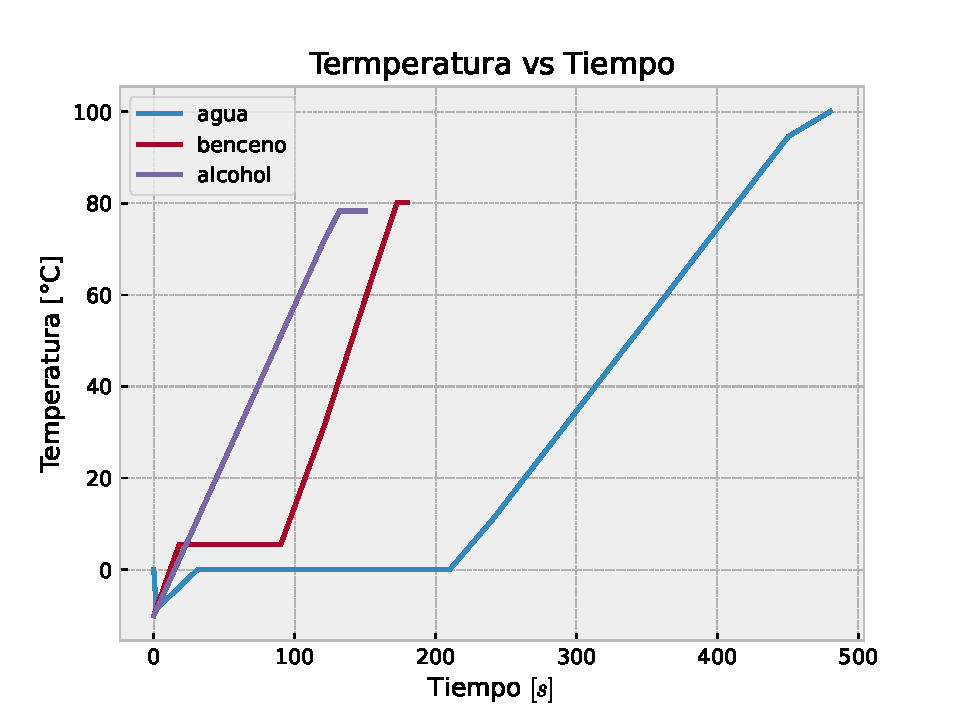
\includegraphics[width=12cm, height=8cm]{ebullicion-fusion/grafico-ebullicion-fusion.pdf}
      \label{img: ebullicion-fusion}      
\end{figure}


\begin{table}[H]
    \centering
 \begin{tabular}{|c|c|c|c|}\hline
                            &  agua &  alcohol  &   benceno  \\ \hline
 Punto de fusión (°C)       &   0   &  N/A      &    5.5      \\ \hline
 Punto de ebullición (°C)   &   100 &    78.3   &    80.2      \\ \hline
    
 \end{tabular}
 \label{tab:ebullicion-fusion2} 
 \caption{ Puntos de fusión y de ebullición.}
\end{table}



\subsection{Masa de una sustancia}
\begin{itemize}
      \item Primero, seleccionaremos una potencia de 500[W], una masa de 100[g] 
      de alcochol y una temperatura inicial de 10°C.
      \item  Segundo, anotaremos la temperatura, al menos 8 valores espaciados. El punto de ebullición no será considerado.
      \item Tercero, repetiremos el experimento para 150[g] y 200[g] de alcohol.
\end{itemize}
Según los datos obtenidos \ref{img: masa} mientras menor sea la masa de la sustancia, más rápido se calentará.

\begin{table}[H]
      \centering
      \begin{tabular}{|c|c|c|}\hline
           Masa [g]& Tiempo [s] & Temperatura [°C]\\ \hline
                   &   0.0      &  10.0\\
                   &   5.1      &  20.3\\
                   &   9.8      &  29.9\\
          100      &   14.3     &  39.0\\
                   &   18.4     &  47.3\\
                   &  22.9      &  56.5 \\
                   &  27.3      &  65.4\\
                   &  31.7      &  74.4\\ \hline
                   & 0.0        &  10.0\\
                   &4.1         &  15.5\\
                   &7.9         &  20.7\\
                   &11.0        &  24.9\\
                   &14.7        &  29.9\\ 
          150      &18.5        &  35.0\\
                   &22.0        &  39.8\\
                   &25.2        &  44.1\\
                   &29.1        &  49.4\\
                   &32.7        &  54.3\\
                   &36.7        &  59.7\\
                   &40.5        &  64.8\\
                   &44.5        &  70.2\\
                   &48.1        &  75.1\\ \hline 
                  &    0.0       &10.0\\
                  &   4.9        &14.9\\
                  &    8.3       &18.4\\
                  &    11.2      &21.3\\
                  &    14.9      &25.1\\
                  &    18.4      &28.6\\
                  &    21.7      &32.0\\
                  &   25.2       &35.6\\
                  &    29.1      &39.5\\
      200         &    33.1      &43.6\\
                  &    36.9      &47.5\\
                  &    41.3      &51.9\\
                  &    44.9      &55.6\\
                  &    50.3      &61.1\\
                  &    53.3      & 64.1\\
                  &    57.3      & 68.2\\
                  &    61.1      &72.0\\
                  &    64.9      &75.9\\ \hline
      \end{tabular}
      \label{tab:masa }
      \caption[]{Datos del experimento: Masa de una sustancia.}
\end{table}

\begin{figure}[H]
      \centering
      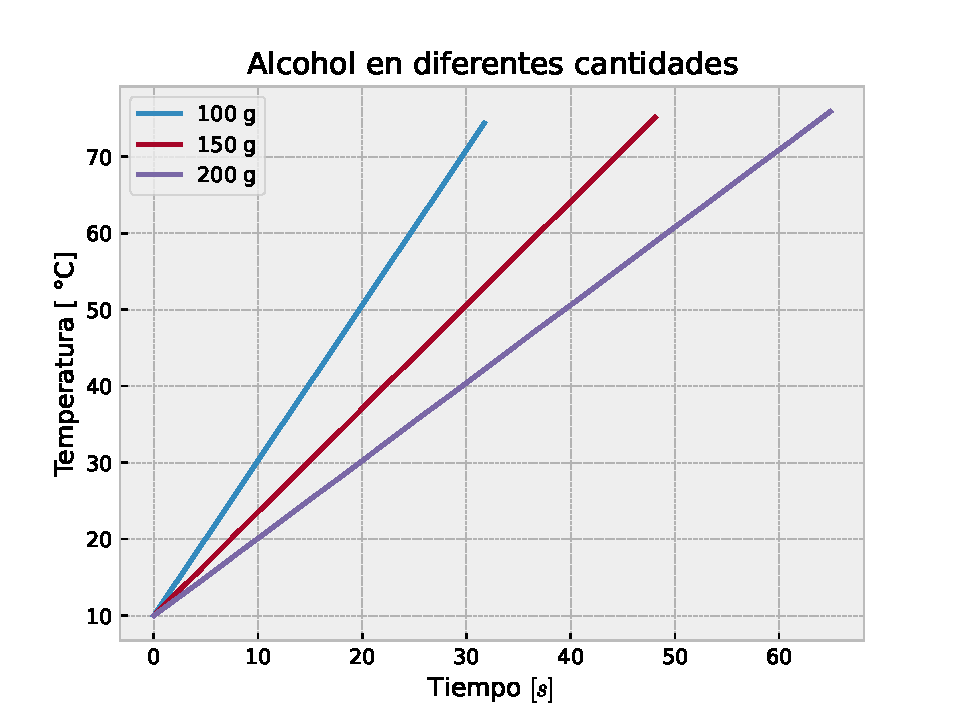
\includegraphics[width=12cm, height=8cm]{masa/grafico-alcohol-masa.pdf}
      \label{img: masa}
\end{figure}



\subsection{Potencia de la estufa}
\begin{itemize}
      \item Primero, seleccionaremos una potencia de 250[W], una masa de 100[g] de benceno y una temperatura inicial de 10°C.
      \item Segundo, anotaremos la temperatura, al menos 8 valores espaciados. El punto de ebullición no será considerado.
      \item Tercero, repetiremos el experimento para 500[W] y 1000[W].
\end{itemize}
Segun los datos obtenidos \ref{img: potencia} a mayor potencia, la sustancia alcanza más rápido su punto de ebullición.


\begin{table}[H]
      \centering
      \begin{tabular}{|c|c|c|}\hline
            Potencia [W]& Tiempo [s] & Temperatura [°C]\\ \hline
                        &   0.0    &10.0\\
                        & 3.7      &15.2\\
                        &8.1        &21.5\\
                        &11.5       &26.4\\
                        &15.7       &32.4\\
            250         &19.4       &37.7\\
                        &22.9        &42.7\\
                        &26.7        &48.1\\
                        &31.1         &54.4\\
                        &35.1         &60.1\\
                        &39.5         &66.4\\
                        &43.7        &72.4\\
                        &48.1        &78.7\\ \hline        
                        &0.0         &10.0\\
                        &3.1        &18.8\\
            500         &6.5        &28.5\\
                        &10.0       &38.5\\
                        &13.1       &47.4\\
                        &16.9       &58.2\\
                        &19.9       &66.8\\
                        &23.0       &75.7\\ \hline
                        &0.0        &10.0\\
                        &1.7        &19.7\\
            1000        &3.3        &28.8\\
                        &4.9        &38.0\\
                        &6.5         &47.1\\
                        &7.9        &55.1\\
                        &9.2         &62.5\\
                        &10.3       &68.8\\
                        &11.5       &75.7\\ \hline    
      \end{tabular}
      \label{tab: potencia}
      \caption[]{Datos del experimento: Potencia de la estufa.}
      
\end{table}
\begin{figure}[H]
      \centering
      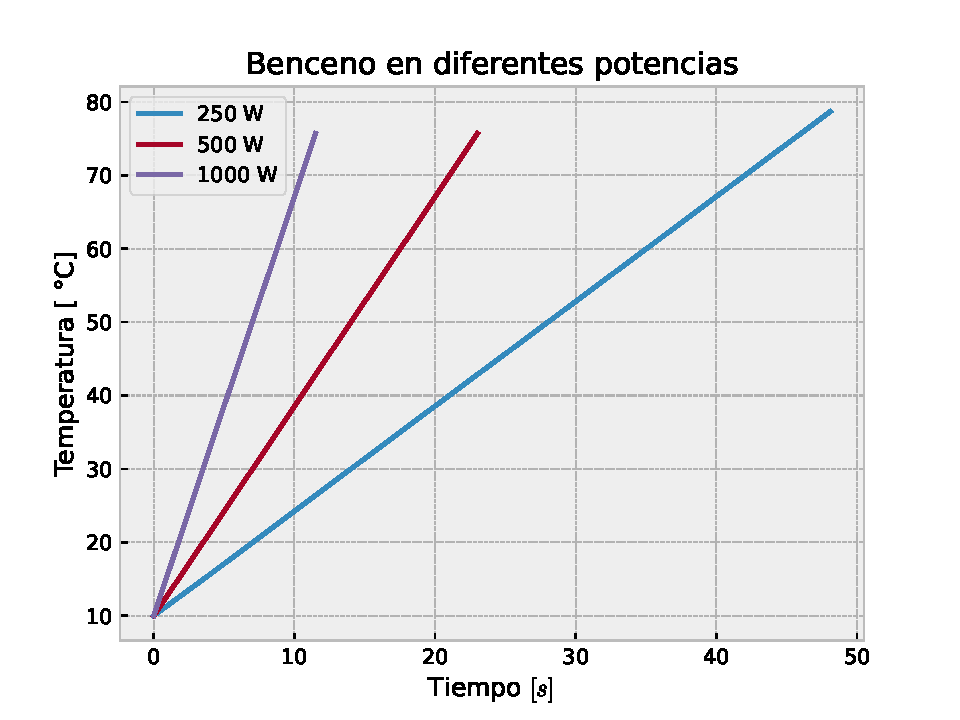
\includegraphics[width=12cm, height=8cm]{potencia/grafico-benceno-potencia.pdf}
      \label{img: potencia}
\end{figure}



\subsection{La naturaleza de la sustancia}
\begin{itemize}
      \item Primero, seleccionaremos una potencia de 250[W], una masa de 150[g] de agua a una temperatura inicial de 0°C.
      \item Segundo, anotaremos la temperatura, al menos 8 valores espaciados. El punto de ebullición, no será considerado.
      \item Tercero, repetiremos el experimento para la sustancia de alcohol y benceno.
\end{itemize}
Según los datos obtenidos \ref{img: naturaleza} el alcohol, a mismas condiciones iniciales, se demora menos en alcanzar su punto de ebullición.

\begin{table}[H]
      \centering
      \begin{tabular}{|c|c|c|}
            Sustancia [W]& Tiempo [s] & Temperatura [°C]\\ \hline
                            &  0.0  &0.0\\
                            & 29.9  &0.0\\
                            & 59.7  &0.0\\
                            & 90.1  &0.0\\
                            & 119.9 &0.0\\
                            & 149.7 &0.0\\
                            & 179.8 &0.0\\
         agua               & 210.3 &3.9\\
                            & 239.9 &15.6\\
                            & 269.9 &27.6\\
                            & 300.0 &39.6\\
                            & 330.0 &51.5\\
                            & 359.9 &63.4\\
                            & 389.9 &75.4\\
                            & 419.5 &87.2\\
                            & 450.3 &99.5\\ \hline
                              & 0.0  & 0.0\\
                              & 14.7 & 9.9\\
                              & 29.9 & 20.2\\
         alcohol              & 45.1 & 30.5\\
                              & 59.9 & 40.5\\
                              & 74.7 & 50.6\\
                              & 89.9 & 60.9\\
                              & 104.7 & 70.9 \\ \hline
                              &0.0  &0.0\\
                              &19.5 &5.5\\
                              &39.7 &5.5 \\
        benceno               &60.1 &5.5\\
                              &79.9 &5.5\\
                              &99.7 &21.8\\
                              &120.1 &41.3\\
                              & 139.8 &60.0\\
                              &159.7 &79.0\\ \hline

      \end{tabular} 
      \label{tab: naturaleza}
      \caption[]{Datos del experimento: La naturaleza de la sustancia.}
\end{table}


\begin{figure}[H]
      \centering
      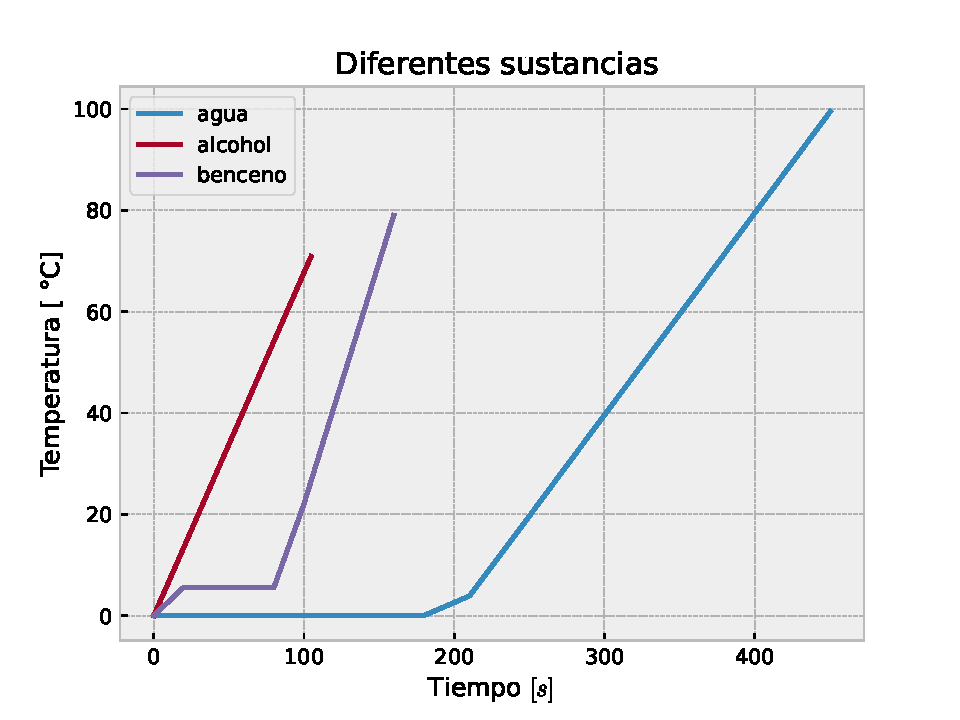
\includegraphics[width=12cm, height=8cm]{naturaleza/grafico-naturaleza-sustancias.pdf}
      \label{img: naturaleza}
\end{figure}



\end{document}